

\section{Durchführung}
\label{sec:Durchführung}
Ziel des Versuches war es, die Dampfdruckkurve von Wasser einmal zwischen $30$ und $1000 \si{\milli\bar}$
und einmal zwischen $1$ und $50 \si{\bar}$. Daraus galt es, die Verdampfungswärme zu bestimmten
sowie deren Temperaturabhängigkeit für $p \geq \si{\bar}$.

\subsection{Niedrige Drücke}
\begin{figure}
    \centering
    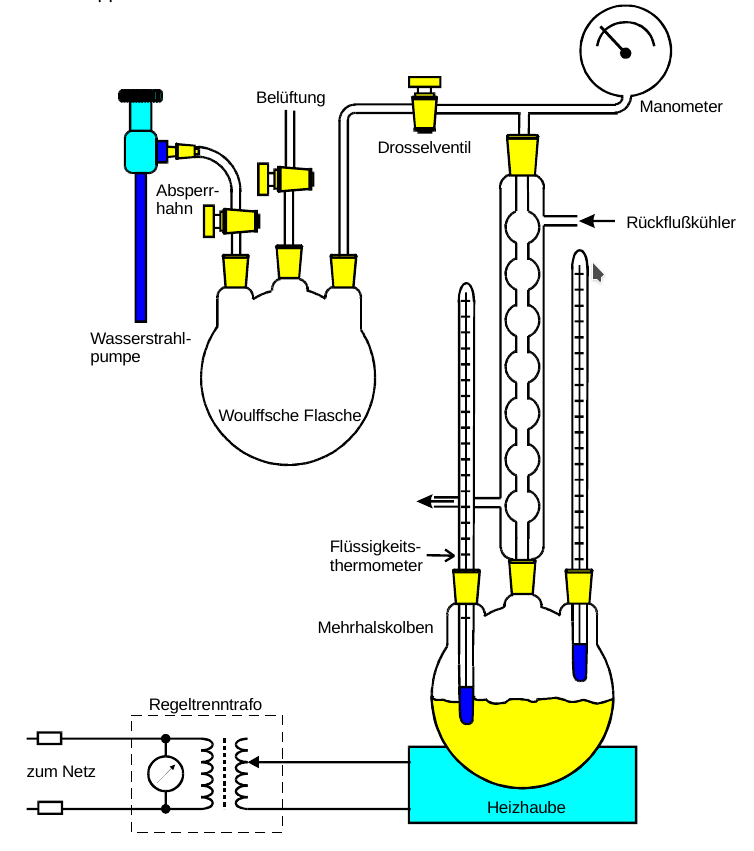
\includegraphics[width=\textwidth]{apparatur1.png}
    \caption{Schematischer Versuchsaufbau zur Messung im Bereich niedriger Drücke.}
    \label{fig:app1}
\end{figure}
Abbildung \ref{fig:app1} zeigt die Apparatur, die genutzt werden kann, um für kleinere Drücke $\symup{p} \leq 1 \si{\bar}$
das Verhältnis zwischen Druck und Temperatur aufzunehmen. \\
Die Woulffsche Flasche dient einerseits dem Evakuieren der Apparatur, zudem soll sie es verhindern,
dass kaltes Wasser in die erhitzte Apparatur einfliesst. Der Rückflusskühler nutzt Kühlwasser, um
aufsteigende Dämpfe zu kondensieren, damit sie nicht ins Manometer strömen. \\
Um den Aufbau auf den Versuch vorzubereiten, wird die Wasserstrahlpumpe zum evakuieren genutzt,
wobei Absperrhahn und Drosselventil geöffnet und das Belüftungsventil geschlossen werden.
Das verbundene Manometerzeigt den Druckabfall an; dessen Ausprägung ist abhängig von der
Temperatur des Leitungswassers, das durch die Wasserstrahlpumpe fliesst. Ist der niedrigste realisierbare
Druck erreicht, werden Absperrhahn un Drosselventil geschlossen und die Heizhaube eingeschaltet.
Zudem muss die Kühlwasserzufuhr gestartet werden, die sollte aber mit zunehmender Temperatur abgeschwächt 
werden, bis sie oberhalb von $80 \si{\degreeCelsius}$ nur noch tropfen soll.\\
In Schritten von $20 \si{\milli\bar}$ wird die entsprechende Temperatur aufgeschrieben.

\subsection{Höhere Drücke}
\begin{figure}
    \centering
    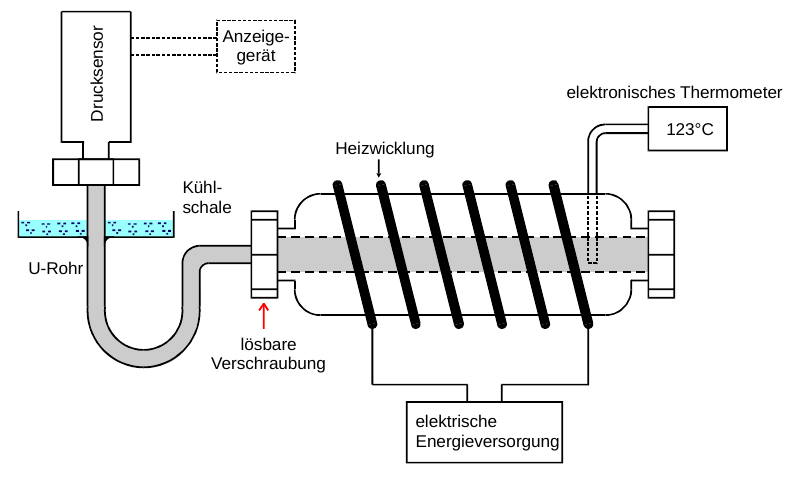
\includegraphics[width=\textwidth]{apparatur2.png}
    \caption{Schematischer Versuchsaufbau zur Messung im Bereich höherer Drücke.}
    \label{fig:app2}
\end{figure}
Eine weitere Apparatur, wie sie in \ref{fig:app2} gezeigt ist, erlaubt die Untersuchung des Zusammenhangs
von Druck und Temperatur bei $\symup{p} \geq 1 \si{\bar}$.\\
Die Heizwicklung, die in der Abbildung gekennzeichnet ist, umgibt einen Stahlzylinder, dessen Inneres
die zu untersuchende Flüssigkeit enthält. Ein U-Rohr verbindet das Innere des Zylinders mit einem Drucksensor
und einem Anzeigegerät, die Verbindung zum Stahlzylinder ist dabei durch eine Bleiplatte 
verdichtet. Durch ein Bohrloch im Zyliner wird ein Thermometer geführt.\\
Bevor die Messung beginnen kann, muss die Apparatur aufgeschraubt und der Zylinder vollständig mit
der zu untersuchenden Substanz gefüllt werden - hier mit entgastem Wasser. Anschließend wird die Heizung
eingeschaltet und in Schritten von $0.5 \si{\bar}$ wird die zugehörige Temperatur abgelesen.